% Drawing 138/07-11 -- folder 138, batch 07, archive page 129 (PDF page 130).
% Transcription: un disque (sphère) traversé d'un arc joignant deux points, numéroté III).
% Kind: disc crossed by an arc. Method 2 (schematic redraw from the facsimile). Status: ok.
% Notes: A disc (the sphere), its upper rim inked over, crossed by a thick arc joining two points; numbered III).
% Coordinates: 1 unit = 1 mm = 1/100 of the crop width (bbox in page fractions: [0.504, 0.441, 0.632, 0.498]).
% Redrawn by Claude (claude-opus-5-5), issue #73, 2026-11-07; not checked by a human; not compiled (no TeX in the session).
% Rights: reproduces part of the work -- behind RENDER_TRANSCRIPTS, never published by itself.
\documentclass[tikz,border=3pt]{standalone}
\usepackage{amsmath,amssymb}
\usetikzlibrary{patterns,arrows.meta}
\tikzset{pencil/.style={black!45}, struck/.style={black!35}, mark/.style={circle,draw,inner sep=1.3pt}, pt/.style={circle,fill,inner sep=0.9pt}, opt/.style={circle,draw,fill=white,inner sep=1.1pt}}
\begin{document}
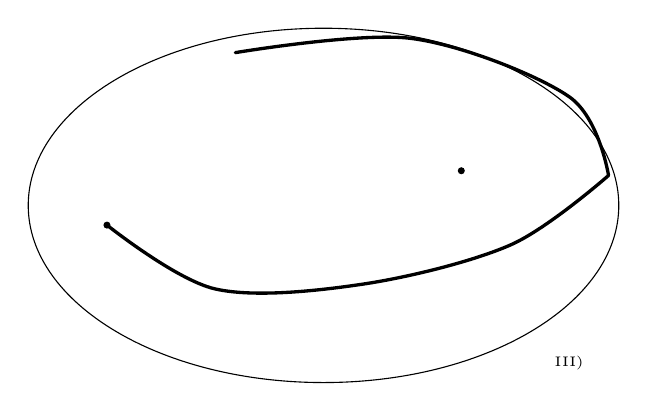
\begin{tikzpicture}[x=1mm,y=1mm,line cap=round,line join=round,font=\scriptsize]
\draw (45,-30) ellipse[x radius=37.5, y radius=22.5];
\draw[very thick] plot[smooth, tension=0.55] coordinates {(33.8,-10.6) (56.2,-8.8) (76.2,-16.2) (81.2,-26.2)};
\draw[very thick] plot[smooth, tension=0.55] coordinates {(17.5,-32.5) (31.2,-40.6) (50,-40) (68.8,-35) (81.2,-26.2)};
\node[pt] at (17.5,-32.5) {};
\node[pt] at (62.5,-25.6) {};
\node[inner sep=1pt] at (76.2,-50) {\tiny III)};
\end{tikzpicture}
\end{document}
